\section[Wykład 3: 9-III-2017 - Temat: Grafy planarne. Minory. Liczba chromatyczna.]{Temat: Grafy planarne. Minory. Liczba chromatyczna.}
\subsection{Definicje grafów planarnych}
\begin{definition}[Graf planarny]
Graf $G=(V,E)$  nazywamy planarny, gdy krawędzie grafu ($E(G)$) się nie przecinają, na przykład:\\
$K_4$: 
\begin{minipage}{.45\textwidth}
\begin{figure}[H]
\centering
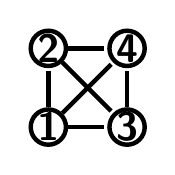
\begin{tikzpicture}[shorten >=1pt, auto, node distance=3cm, ultra thick,main node/.style={circle,draw,minimum size=.4cm,inner sep=0pt]}]%fill=black,
\begin{scope}[every node/.style={font=\sffamily\Large\bfseries}]
\node[main node] (v1) at (0,0) {1};
\node[main node] (v2) at (0,1) {2};
\node[main node] (v3) at (1,0) {3};
\node[main node] (v4) at (1,1) {4};
\end{scope}
\begin{scope}
\draw  (v1) edge node{} (v2);
\draw  (v1) edge node{} (v3);
\draw  (v1) edge node{} (v4);
\draw  (v2) edge node{} (v3);
\draw  (v2) edge node{} (v4);
\draw  (v3) edge node{} (v4);
\end{scope}
\end{tikzpicture}
\end{figure}
\end{minipage}
\begin{minipage}{.45\textwidth}
\begin{figure}[H]
\centering
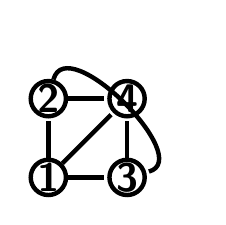
\begin{tikzpicture}[shorten >=1pt, auto, node distance=3cm, ultra thick,main node/.style={circle,draw,minimum size=.4cm,inner sep=0pt]}]%fill=black,
\begin{scope}[every node/.style={font=\sffamily\Large\bfseries}]
\node[main node] (v1) at (0,0) {1};
\node[main node] (v2) at (0,1) {2};
\node[main node] (v3) at (1,0) {3};
\node[main node] (v4) at (1,1) {4};
\end{scope}
\begin{scope}
\draw  (v1) edge node{} (v2);
\draw  (v1) edge node{} (v3);
\draw  (v1) edge node{} (v4);
\draw[bend left=120]  (v2) edge node{} (v3);
\draw  (v2) edge node{} (v4);
\draw  (v3) edge node{} (v4);
\end{scope}
\end{tikzpicture}
\end{figure}
\end{minipage}
\end{definition}

\begin{definition}[Grafy planarne] Grafy planarne $\rightarrow$ graf, który można narysować w taki sposób aby krawędzie się nie przecinały (z wyjątkiem wierzchołków).
\end{definition}
{
%ŚCIĄGA: http://tex.stackexchange.com/questions/29246/factorial-design-diagrams-in-tikz
\newcommand\drawplane[2]
{%
    \draw
    [
        thick,
        opacity=.6,
        draw=#2,
        fill=#2!60,
    ] #1 -- cycle;%
}

\newcommand\drawonecase[4]
{
    \begin{tikzpicture}[scale=2]

        \tikzset
        {
            edgevis/.style={black},
            edgehid/.style={dashed,black},
        }

        \def\vertexradius{.7pt}

        \coordinate (OOO) at (0,0);
        \coordinate (OOI) at (xyz cs:z=1);
        \coordinate (OIO) at (xyz cs:y=1);
        \coordinate (OII) at (xyz cs:y=1,z=1);
        \coordinate (IOO) at (xyz cs:x=1);
        \coordinate (IOI) at (xyz cs:x=1,z=1);
        \coordinate (IIO) at (xyz cs:x=1,y=1);
        \coordinate (III) at (xyz cs:x=1,y=1,z=1);

        \drawplane{#1}{#2}
        \drawplane{#3}{#4}

        \draw[edgevis] (OOI) -- (OII) -- (OIO) -- (IIO) -- (IOO) -- (IOI) -- cycle;
        \draw[edgevis] (III) -- (IIO);
        \draw[edgevis] (III) -- (IOI);
        \draw[edgevis] (III) -- (OII);
        \draw[edgehid] (OOO) -- (OOI);
        \draw[edgehid] (OOO) -- (OIO);
        \draw[edgehid] (OOO) -- (IOO);

        \draw (OOO) circle (\vertexradius);
        \draw (OOI) circle (\vertexradius);
        \draw (OIO) circle (\vertexradius);
        \draw (OII) circle (\vertexradius);
        \draw (IOO) circle (\vertexradius);
        \draw (IOI) circle (\vertexradius);
        \draw (IIO) circle (\vertexradius);
        \draw (III) circle (\vertexradius);

    \end{tikzpicture}
}
$Q_4$:
\begin{minipage}{.48\textwidth}
\begin{figure}[H]
\centering
\drawonecase
                {(OOO) -- (OOI) -- (OII) -- (OIO)}{red}
                {(IOO) -- (IOI) -- (III) -- (IIO)}{blue}
\end{figure}
\end{minipage}
\begin{minipage}{.48\textwidth}
\begin{figure}[H]
\centering
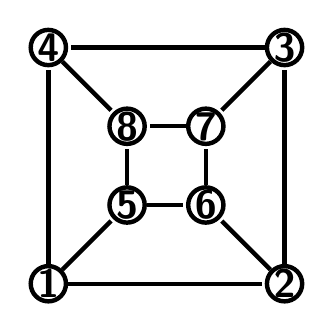
\begin{tikzpicture}[shorten >=1pt, auto, node distance=3cm, ultra thick,main node/.style={circle,draw,minimum size=.4cm,inner sep=0pt]}]%fill=black,
\begin{scope}[every node/.style={font=\sffamily\Large\bfseries}]
\node[main node] (v1) at (0,0) {1};
\node[main node] (v2) at (3,0) {2};
\node[main node] (v3) at (3,3) {3};
\node[main node] (v4) at (0,3) {4};
\node[main node] (v5) at (1,1) {5};
\node[main node] (v6) at (2,1) {6};
\node[main node] (v7) at (2,2) {7};
\node[main node] (v8) at (1,2) {8};
%\node[main node] (v) at (,) {};
\end{scope}
\begin{scope}
\draw  (v1) edge node{} (v2);
\draw  (v1) edge node{} (v4);
\draw  (v1) edge node{} (v5);
\draw  (v2) edge node{} (v3);
\draw  (v2) edge node{} (v6);
\draw  (v3) edge node{} (v4);
\draw  (v3) edge node{} (v7);
\draw  (v4) edge node{} (v8);
\draw  (v5) edge node{} (v6);
\draw  (v5) edge node{} (v8);
\draw  (v6) edge node{} (v7);
\draw  (v7) edge node{} (v8);
%\draw  (v) edge node{} (v);
\end{scope}
\end{tikzpicture}
\end{figure}
\end{minipage}
}

\begin{definition}[Graf płaski] Grafem płaskim nazywamy dowolny rysunek grafu planarnego, w którym żadna krawędź nie ma punktów wspólnych (za wyjątkiem punktów wierzchołków) z inną krawędzią. 
\end{definition}

\begin{definition}[kopia topologiczna] Graf $G'$ jest kopią topologiczną grafu $G$ jeżeli $G'$ powstaje z $G$ przez zastąpienie niektórych krawędzi ścieżkami (dowolnej długości). 
\begin{minipage}{.48\textwidth}
\begin{figure}[H]
\centering
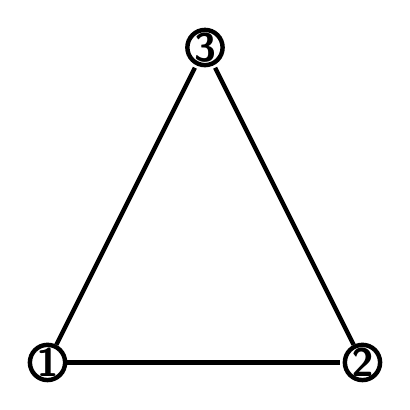
\begin{tikzpicture}[shorten >=1pt, auto, node distance=3cm, ultra thick,main node/.style={circle,draw,minimum size=.4cm,inner sep=0pt]}]%fill=black,
\begin{scope}[every node/.style={font=\sffamily\Large\bfseries}]
\node[main node] (v1) at (0,0) {1};
\node[main node] (v2) at (4,0) {2};
\node[main node] (v3) at (2,4) {3};
%\node[main node] (v) at (,) {};
\end{scope}
\begin{scope}
\draw  (v1) edge node{} (v2);
\draw  (v1) edge node{} (v3);
\draw  (v2) edge node{} (v3);
%\draw  (v) edge node{} (v);
\end{scope}
\end{tikzpicture}
\caption*{$C_3$}
\end{figure}
\end{minipage}
\begin{minipage}{.48\textwidth}
maksymalna liczn\begin{figure}[H]
\centering
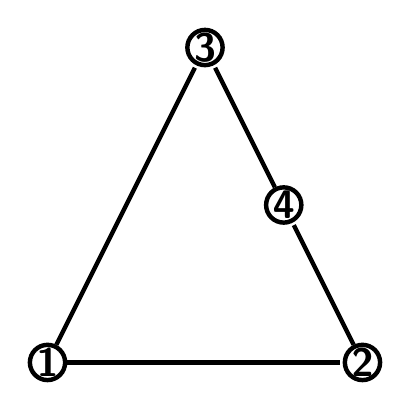
\begin{tikzpicture}[shorten >=1pt, auto, node distance=3cm, ultra thick,main node/.style={circle,draw,minimum size=.4cm,inner sep=0pt]}]%fill=black,
\begin{scope}[every node/.style={font=\sffamily\Large\bfseries}]
\node[main node] (v1) at (0,0) {1};
\node[main node] (v2) at (4,0) {2};
\node[main node] (v3) at (2,4) {3};
\node[main node] (v4) at (3,2) {4};
%\node[main node] (v) at (,) {};
\end{scope}
\begin{scope}
\draw  (v1) edge node{} (v2);
\draw  (v1) edge node{} (v3);
\draw  (v2) edge node{} (v4);
\draw  (v4) edge node{} (v3);
%\draw  (v) edge node{} (v);
\end{scope}
\end{tikzpicture}
\caption*{$C_4$ będący topologiczną kopią $C_3$}
\end{figure}
\end{minipage}
\end{definition}

\begin{definition}[Grafy homeomorficzne]
graf $G_1$ jest homeomorficzny z $G_2$, jeśli jeden można otrzymać z drugiego poprzez wykonanie skończenie wielu z poniższych operacji:
\begin{description}
\item[dodawanie wierzchołków stopnia dwa na krawędzi] – jeśli $uw \in E (G_1)$ oraz $x \not \in V (G_1)$, to operacja ta zastępuje graf $(V (G_1), E (G_1))$ grafem $(V (G_1) \cup \{x\} , E (G_1) \cup \{ux, xw\} - \{uw\})$;
\item[usuwanie wierzchołków stopnia dwa] – jeśli $x\in V (G_1)$ ma jedynie dwóch sąsiadów $u, w$, to operacja ta zastępuje graf $(V (G_1), E (G_1))$ grafem $(V (G_1) - \{x\} , E (G_1) \cup \{uw\} - \{ux, xw\})$.
\end{description}
\end{definition}

\begin{fact*}
Jeśli $G'$ jest kopią topologiczną $G$ to $G$ jest planarny wtedy i tylko wtedy, gdy $G'$ jest planarny.
\end{fact*}

\begin{theorem}[Kuratowski]\label{the:Kuratowski}
Graf $G$ jest planarny wtedy i tylko wtedy, gdy $G$ nie zawiera kopii topologicznych grafów:
\begin{itemize}
\item $K_5$
\item $K_{3,3}$
\end{itemize}
\end{theorem}

\begin{definition}[Minor grafu]
Graf $G$ zawiera graf $H$ jako minor: $G\triangleright H$ jeśli $H$ można otrzymać z $G$ za pomocą następujących operacji:
\begin{itemize}
\item usuwania wierzchołków, krawędzi,
\item ściągania krawędzi\\
\begin{minipage}{.30\textwidth}
\begin{figure}[H]
\centering
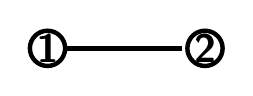
\begin{tikzpicture}[shorten >=1pt, auto, node distance=3cm, ultra thick,main node/.style={circle,draw,minimum size=.4cm,inner sep=0pt]}]%fill=black,
\begin{scope}[every node/.style={font=\sffamily\Large\bfseries}]
\node[main node] (v1) at (0,0) {1};
\node[main node] (v2) at (2,0) {2};
\end{scope}
\begin{scope}
\draw  (v1) edge node{} (v2);
\end{scope}
\end{tikzpicture}
\end{figure}
\end{minipage}$\rightarrow$
\begin{minipage}{.30\textwidth}
\begin{figure}[H]
\centering
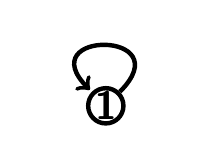
\begin{tikzpicture}[shorten >=1pt, auto, node distance=3cm, ultra thick,main node/.style={circle,draw,minimum size=.4cm,inner sep=0pt]}]%fill=black,
\begin{scope}[every node/.style={font=\sffamily\Large\bfseries}]
\node[main node] (v1) at (0,0) {1};
\end{scope}
\begin{scope}
\draw[loop]  (v1) edge node{} (v1);
\end{scope}
\end{tikzpicture}
\end{figure}
\end{minipage}$\rightarrow$
\begin{minipage}{.30\textwidth}
\begin{figure}[H]
\centering

\begin{tikzpicture}[shorten >=1pt, auto, node distance=3cm, ultra thick,main node/.style={circle,draw,minimum size=.4cm,inner sep=0pt]}]%fill=black,
\begin{scope}[every node/.style={font=\sffamily\Large\bfseries}]
\node[main node] (v1) at (0,0) {1};
\end{scope}
\begin{scope}
\end{scope}
\end{tikzpicture}
\end{figure}
\end{minipage}
\end{itemize}
\end{definition}

\begin{definition}[Ściągnięcie grafu]
Mówimy, że graf $G|_e$ jest \textbf{ściągnięciem} grafu $G$ wzdłuż krawędzi $e = uv$, jeśli:
\begin{itemize}
\item[] $V (G|_e) = V (G) - \{u, v\} \cup \{x\}$ dla $x \not \in V (G)$ oraz
\item[] $E (G|_e) = E (G - \{u, v\})\cup \{xw\}$ dla każdego wierzchołka $w \in V (G-\{u, v\})$ takiego, że $uw \in E(G)$ lub $vw \in E(G)$.
\end{itemize}
\end{definition}

\begin{fact*}
Jeśli $G$ jest planarny i $G\triangleright H$ to $H$ też jest planarny.
\end{fact*}

\begin{theorem}[Wagner]\label{the:Wagner} Graf $G$ jest planarny wtedy i tylko wtedy, gdy $G\not \triangleright K_5$ i $G\not \triangleright K_{3,3}$
\end{theorem}

\begin{theorem}[Robertson, Seymour]\label{the:RobertsonSeymour} Dla dowolnego grafu $H$ istnieje stała $c_H$ i algorytm $\mathcal{A}_H$, który w czasie nie większym niż $c_H n^3$ sprawdza, czy ustalony graf na $n$ wierzchołkach zawiera $H$ jako minor.
\end{theorem}
\begin{remark}
Umiemy w czasie wielomianowym (od 1 wierzchołka) sprawdzić, czy dany graf jest planarny.
\end{remark}

\textbf{UWAGA!} Graf planarny może mieć wiele płaskich reprezentacji.\\
\begin{minipage}{.4\textwidth}
\begin{figure}[H]
\centering
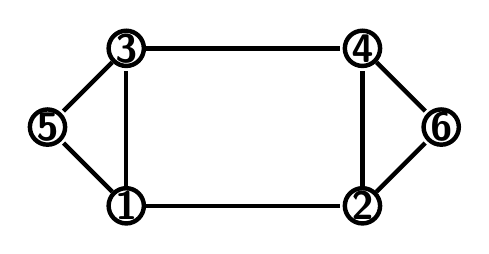
\begin{tikzpicture}[shorten >=1pt, auto, node distance=3cm, ultra thick,main node/.style={circle,draw,minimum size=.4cm,inner sep=0pt]}]%fill=black,
\begin{scope}[every node/.style={font=\sffamily\Large\bfseries}]
\node[main node] (v1) at (0,0) {1};
\node[main node] (v2) at (3,0) {2};
\node[main node] (v3) at (0,2) {3};
\node[main node] (v4) at (3,2) {4};
\node[main node] (v5) at (-1,1) {5};
\node[main node] (v6) at (4,1) {6};
%\node[main node] (v) at (,) {};
\end{scope}
\begin{scope}
\draw  (v1) edge node{} (v2);
\draw  (v1) edge node{} (v3);
\draw  (v1) edge node{} (v5);
\draw  (v2) edge node{} (v4);
\draw  (v2) edge node{} (v6);
\draw  (v3) edge node{} (v4);
\draw  (v3) edge node{} (v5);
\draw  (v4) edge node{} (v6);
%\draw  (v) edge node{} (v);
\end{scope}
\end{tikzpicture}
\end{figure}
\end{minipage}
\begin{minipage}{.4\textwidth}
\begin{figure}[H]
\centering
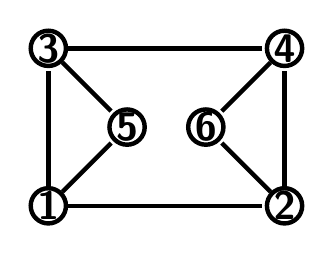
\begin{tikzpicture}[shorten >=1pt, auto, node distance=3cm, ultra thick,main node/.style={circle,draw,minimum size=.4cm,inner sep=0pt]}]%fill=black,
\begin{scope}[every node/.style={font=\sffamily\Large\bfseries}]
\node[main node] (v1) at (0,0) {1};
\node[main node] (v2) at (3,0) {2};
\node[main node] (v3) at (0,2) {3};
\node[main node] (v4) at (3,2) {4};
\node[main node] (v5) at (1,1) {5};
\node[main node] (v6) at (2,1) {6};
%\node[main node] (v) at (,) {};
\end{scope}
\begin{scope}
\draw  (v1) edge node{} (v2);
\draw  (v1) edge node{} (v3);
\draw  (v1) edge node{} (v5);
\draw  (v2) edge node{} (v4);
\draw  (v2) edge node{} (v6);
\draw  (v3) edge node{} (v4);
\draw  (v3) edge node{} (v5);
\draw  (v4) edge node{} (v6);
%\draw  (v) edge node{} (v);
\end{scope}
\end{tikzpicture}
\end{figure}
\end{minipage}

\begin{definition}[Ściana grafu] Ścianą grafu płaskiego nazywamy spójny obszar płaszczyzny, który określają (,,wycinają'' jego krawędzie
\begin{description}
\item[$f(G)$] liczba ścian grafu $G$
\item[$f\in F$] zbiór ścian grafu
\item[$d(F)$]  stopień ściany $f$  - liczba krawędzi granicząca z daną ścianą
\begin{figure}[H]
\centering
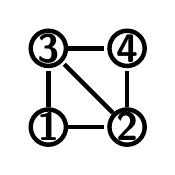
\begin{tikzpicture}[shorten >=1pt, auto, node distance=3cm, ultra thick,main node/.style={circle,draw,minimum size=.4cm,inner sep=0pt]}]%fill=black,
\begin{scope}[every node/.style={font=\sffamily\Large\bfseries}]
\node[main node] (v1) at (0,0) {1};
\node[main node] (v2) at (1,0) {2};
\node[main node] (v3) at (0,1) {3};
\node[main node] (v4) at (1,1) {4};
%\node[main node] (v) at (,) {};
\end{scope}
\begin{scope}
\draw  (v1) edge node{} (v2);
\draw  (v1) edge node{} (v3);
\draw  (v2) edge node{} (v3);
\draw  (v2) edge node{} (v4);
\draw  (v3) edge node{} (v4);
%\draw  (v) edge node{} (v);
\end{scope}
\end{tikzpicture}
\caption*{Przykład: dwie wewnętrzne ściany mają stopień $3$, nieskończona (zewnętrzna) ściana ma stopień $4$ }
\end{figure}
\end{description}
\end{definition}

\begin{theorem}[Euler]\label{the:Euler}
Jeśli graf $G=(V,E)$ jest spójnym grafem płaskim to prawdziwy jest wzór: 
$$\underbrace{V(G)}_\text{liczba wierzchołków} - \underbrace{E(G)}_\text{liczba krawędzi} + \underbrace{f(G)}_\text{liczba ścian} = 2$$
\end{theorem}
\begin{remark}
Wszystkie grafy płaskie danego spójnego grafu planarnego mają tyle samo ścian.
\end{remark}
\begin{fact}
Jeżeli $G$ jest grafem płaskim to: 
$$\sum _{f\in F(G)} d(f)=2E(G)$$
\end{fact}

\begin{theorem}
Jeżeli graf $G$ jest spójnym, prostym grafem planarnym i $|V(G)|\geq 3$ to
$$E(G)\leq 3 V(G)-6$$
\end{theorem}
\begin{remark}
Graf $K_5$ nie jest planarny
\end{remark}

\begin{theorem}
Jeżeli graf $G$ jest prosty, spójnym grafem planarnym nie zawierającym trójkątów to:
$$E(G) \leq 2 V(G) - 4$$
\end{theorem}
\begin{remark}
Graf $K_{3,3}$ nie jest planarny, gdyż: \\
$E(K_{3,3})= 9$m i $2*V(K_{3,3})-4=2*6-4=8$
$$E(K_{3,3})\not \leq 2V(K_{3,3})-4$$
\end{remark}

\subsection{Kolorowanie grafów}
\begin{definition}[$k$-kolorowanie] 
$k$-kolorowaniem wierzchołków grafu $G$ nazywamy funkcję: 
$$c: V\rightarrow\{1,2,..,k\} \text{ kolory}$$
taką, że je:
$$\{v,w\}\in E(G)\text{, to } c(v)\neq c(w)$$
Graf jest $k$-kolorowany, jeśli istnieje jego $k$-kolorowanie
\end{definition}

\begin{definition}[Liczba chromatyczna]
Liczbą chromatyczną grafu $G$ najmniejsze $k$ takie, że graf $G$ jest $k$-kolorowany
$$\chi (G)\rightarrow\text{ liczba chromatyczna}$$
$k$-kolorowanie to podział zbioru wierzchołków $V$ na $k$ podzbiorów $V_1, V_2,..,V_k$ tak, że $V_i$ to zbiór niezależny\footnote{Zbiór niezależny to zbiór w którym, żadne dwa wierzchołki nie są połączone krawędzią.}.
\end{definition}
\begin{remark}
Graf dwudzielny jest $2$-kolorowany
$$\chi (G) \leq \Delta (G)+1$$
\end{remark}

\begin{hipoterm}[Hadwigera]
Jeśli $\chi (G)\geq k$, to $G\triangleright K_k$.
\end{hipoterm}

\begin{theorem}[Twierdzenie o czterech barwach]\label{the:4barwy} 
Jeśli graf $G$ jest planarny, to $$\chi (G) \leq 4$$
\end{theorem}

\begin{definition}[Kolorowanie właściwe]
Kolorowanie wierzchołków jest właściwe, jeśli żadne dwa różne wierzchołki nie są tego samego koloru.
\end{definition}

\begin{definition}[Klika] 
Klika to graf, w którym wszystkie pary wierzchołków są połączone krawędzią (ile ma krawędzi?). Klikę o $n$ wierzchołkach oznaczamy $K_n$.
\end{definition}

%--------------------------------------------------